\section{Эксперименты}
В рамках данной работы были произведены эксперименты по сравнению алгоритмов синтаксического анализа регулярных множеств для на основе алгоритма RNGLR и GLL. 

Замеры производились на компьютере со следующими характеристиками.
\begin{itemize}
\item Операционная система: Microsoft Windows 8.1 Pro.
\item Тип системы: х64-based PC.
\item Процессор: Intel(R) Core(TM) i7-4790 CPU 3.60GHz, 3601 Mhz, 4 Core(s), 8 Logical Processor(s).
\item Объём оперативной памяти: 16.0 GB.
\end{itemize}

Для сравнения были выбраны несколько грамматик, представляющих как практический, так и теоретический интерес. Одна из таких грамматик --- сильно неоднозначная грамматика $G_5$ (листинг~\ref{grmG5}), реализующая худший случай для анализатора, и позволяющая оценить производительность алгоритмов в задачах биоинформатики, так как большинство шаблонов в них являются сильно неоднозначными. Результаты измерений представлены на рис.~\ref{exp1}. 

\begin{listing}
\caption{Грамматика $G_5$}
\label{grmG5}
\centering
$\begin{array}{rl}
s \rightarrow s \ s \ s \ |  \ s \ s \ | \ B 
\end{array}$
\end{listing} 

\begin{figure}
 \centering
 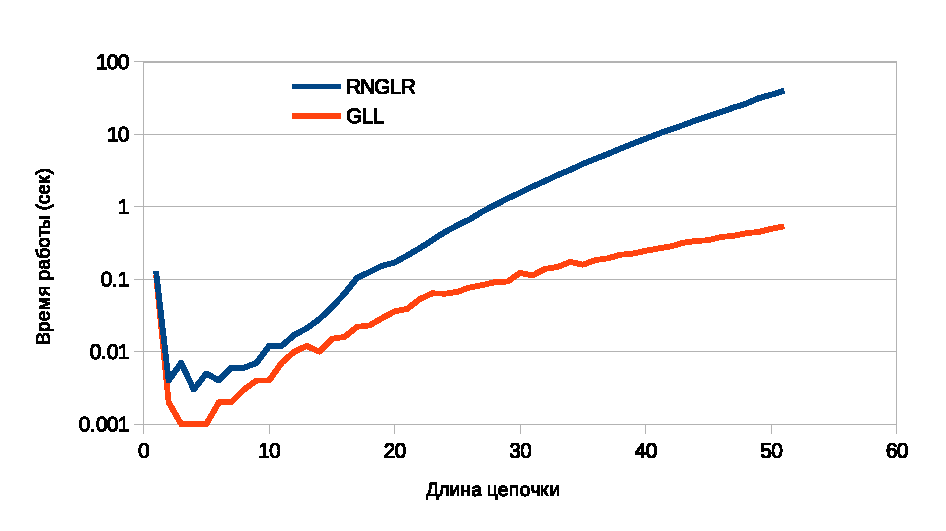
\includegraphics[width=\textwidth]{Ragozina/pics/UmbLog.pdf}
 \caption{Сравнение времени работы решений на основе алгоритмов GLL и RNGLR для грамматики $G_5$}
 \label{exp1}
\end{figure}

Следующей рассматриваемой грамматикой является неоднозначная грамматика правильных скобочных последовательностей $G_6$ (листинг ~\ref{grmG6}). Данная грамматика представляет интерес с практический точки зрения, так как она близка к шаблонам для поиска, используемым в задачах биоинформатики. 

\begin{listing}
\caption{Грамматика $G_6$}
\label{grmG6}
\centering
$\begin{array}{rl}
s \rightarrow s \ s \ |  \ LBR \ s \ RBR \ | \ \varepsilon 
\end{array}$
\end{listing}

Результаты измерений представлены на рис.~\ref{exp2}. Видно, что время работы алгоритма на основе RNGLR растёт значительно быстрее, чем алгоритма на основе GLL, с ростом длины входной цепочки. 

\begin{figure}
 \centering
 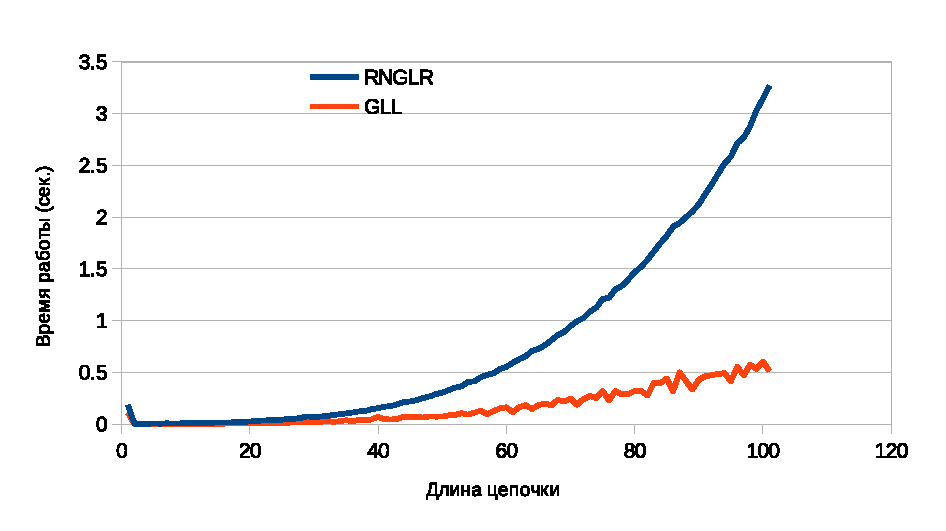
\includegraphics[width=\textwidth]{Ragozina/pics/Brs.pdf}
 \caption{Сравнение времени работы решений на основе алгоритмов GLL и RNGLR для грамматики $G_6$}
 \label{exp2}
\end{figure}

Следующий эксперимент производился на грамматике подмножества языка T-SQL~\cite{YCZOO} . Входные графы строились с помощью последовательной конкатенации блоков с параллельными путями, которые соответствуют использованию операторов ветвления при построении выражения. Пример входного графа приведён на рис.~\ref{SQLInp}.

\begin{figure}
 \centering
 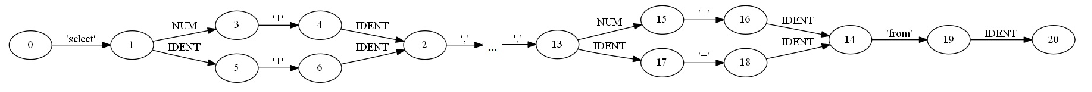
\includegraphics[width=\textwidth]{Ragozina/pics/SQLInput}
 \caption{Структура графа для экспериментов на грамматике T-SQL}
 \label{SQLInp}
\end{figure}

\begin{figure}
 \centering
 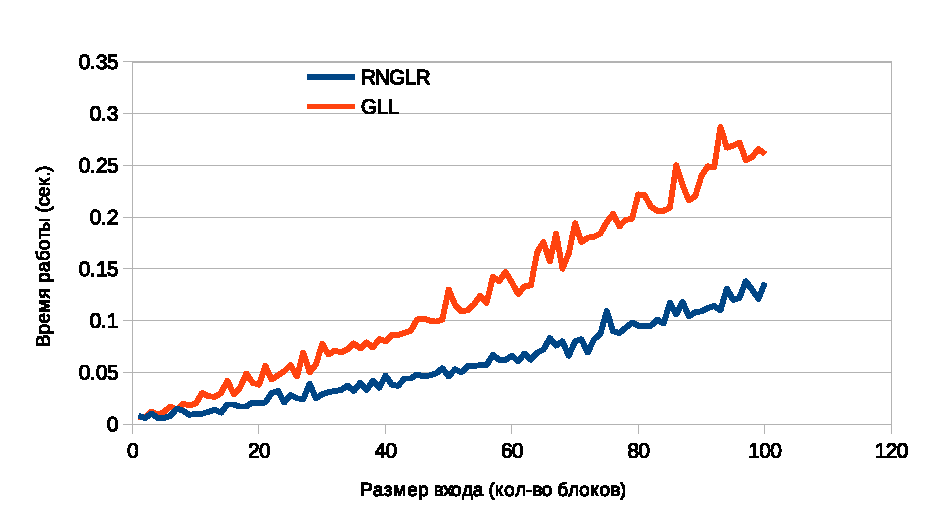
\includegraphics[width=\textwidth]{Ragozina/pics/SQL.pdf}
 \caption{Сравнение времени работы решений на основе алгоритмов GLL и RNGLR для грамматики T-SQL}
 \label{exp3}
\end{figure}

Результаты измерений приведены на рис.~\ref{exp3} В данном случае GLL оказался медленнее. Однако необходимо заметить, что, с одной стороны, на входах практически значимой длины замедление несущественно, а с другой, алгоритм на основе GLR длительное время оптимизировался. Техническая доработка GLL может позволить улучшить его производительность.

Также было проведено сравнение алгоритмов на основе RNGLR и GLL на задаче поиска подцепочки в геноме. В качестве искомой подцепочки была выбрана транспортная РНК, шаблон для поиска которой был описан грамматикой, представленной на листинге~\ref{lst:csqlExample}. Данная грамматика является сильно неоднозначной. В качестве входа была выбрана последовательность из тестов инструмента Infernal~\cite{Infernal} от которой последовательно брались участки длины $100 + 10*k$, начинающиеся с нулевой позиции. Таким образом был получен набор тестовых данных: множество цепочек с увеличивающейся длиной.

\begin{listing}
    \begin{pyglist}[language=ocaml,numbers=left,numbersep=5pt]

stem<s>: 
      A stem<s> U | U stem<s> A
    | C stem<s> G | G stem<s> C
    | G stem<s> U | U stem<s> G
    | s

any: A | U | G | C

[<Start>]
full: folded any?
                        
folded: stem<(any*[1..3] stem<any*[7..10]> 
              any*[1..3] stem<any*[5..8]> 
              any*[3..6] 
              stem<any*[5..8]>)> 

\end{pyglist}
\caption{Пример грамматики для описания транспортной РНК}
\label{lst:csqlExample}
\end{listing}

\begin{figure}
 \centering
 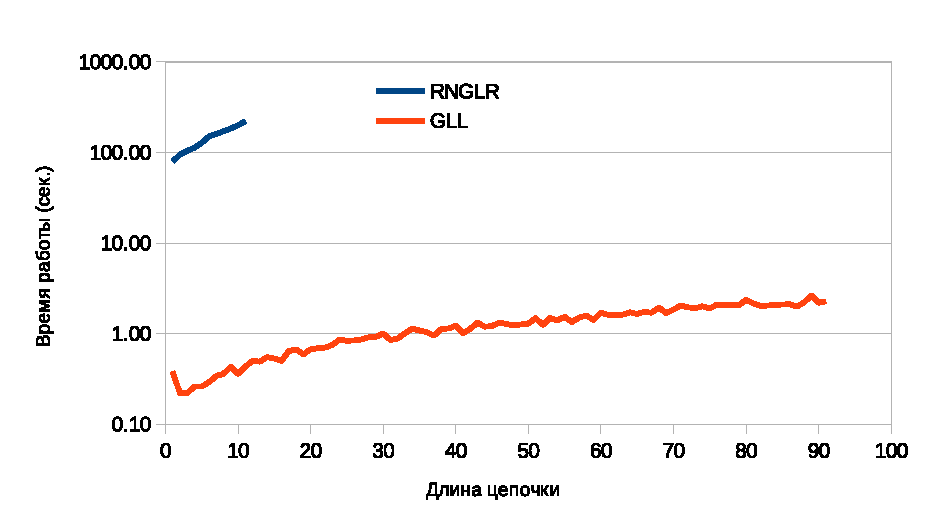
\includegraphics[width=\textwidth]{Ragozina/pics/BioLog.pdf}
 \caption{Сравнение времени работы решений на основе алгоритмов GLL и RNGLR для грамматики на листинге~\ref{lst:csqlExample}}
 \label{fig:Stack}
\end{figure}

График зависимости времени работы от длины цепочки приведён на рис.~\ref{fig:Stack}. Для RNGLR приведены первые 10 замеров, так как дальнейшие измерения для алгоритма на основе RNGLR было решено прекратить из-за его низкой производительности. Приведённые результаты показывают, что реализованный в рамках данной работы алгоритм более чем в 400 раз быстрее алгоритма на основе RNGLR, что согласуется с результатами сравнений на сильно неоднозначной грамматике.
